\section{Soporte de etapas en los flujos de trabajo}
\begin{table}[H]
\centering
\caption{Historias de usuario para soporte de etapas en los flujos de trabajo}
\label{epic:8}
\resizebox{\columnwidth}{!}{%
\begin{tabular}{@{}lllll@{}}
\toprule
Historias de usuario                                             & HE  & HC  & PH & Sprints \\ \midrule
Roles de creación y edición para las partes de flujos de trabajo & 102 & 112 & 13 & 1       \\
Diseño e implementación de etapas                                & 288 & 505 & 21 & 3       \\
Mejora en comportamientos para las etapas por roles              & 84  & 108 & 8  & 2       \\
Composición de etapas y partes                                   & 216 & 391 & 13 & 3       \\
Etapas y partes opcionales en la revisión del flujo              & 64  & 76  & 8  & 1       \\ \bottomrule
\end{tabular}
}
\end{table}

\subsection{Roles de creación y edición para las partes de flujos de trabajo}
La historia de usuario tiene como descripción lo siguiente \enquote{\textit{Como participante en el proceso curricular, podría no solo revisar nuevos cursos y programas, sino que también realizar pequeñas revisiones como parte del proceso o participe también en el paso de compleción del formulario}}.

Como criterios de aceptación se encuentran los siguientes:
\begin{itemize}
	\item Diseñar el privilegio de creador que permitan a un iniciador de flujo o un diseñador de flujo que designe a ciertos roles para escribir o llenar cada paso.
	\item Diseñar el privilegio de editor que permita editar partes a los que revisan el flujo de trabajo antes de aceptar o rechazar.
	\item Configurar flujos de trabajo para que en cada parte o etapa de un flujo de trabajo puedan ser asignados por roles para la tarea de creador o evaluador, o ambos.
\end{itemize}

Algunas de las tareas identificadas en la planificación de las iteraciones eran los siguientes:
\begin{itemize}
	\item Diseñar e implementar nuevos modelos de datos que permitan soportar el uso de roles para creadores y editores de partes.
	\item Diseñar e implementar servicios de visualización para las diferentes secciones de flujos de trabajo.
	\item Actualizar las plantillas de flujo de trabajo para agregar el soporte de roles de creación y edición.
	\item Actualizar el flujo de trabajo para soportar la compleción de secciones por paso.
	\item Implementar la funcionalidad de edición.
\end{itemize}

La historia fue finalizada en tres iteraciones con una cantidad de 112 horas cargadas en el sistema.


\subsection{Diseño e implementación de Etapas}
La historia de usuario tiene como descripción lo siguiente \enquote{\textit{Como administrador curricular quiero ser capaz de configurar mi plantilla de flujo de trabajo para que pueda dividir en etapas donde se especifiquen que roles pueden completar que funciona en una o múltiples secciones o partes de mi programa o curso}}. Y los criterios de aceptación consistían en el desarrollo de la pantalla que se puede apreciar en la figura \ref{visualize_changes}.

Como criterios de aceptación se encuentran los siguientes:
\begin{itemize}
	\item En un diseño de flujo de trabajo se debe elegir un rol, sección o parte y la acción (completar, revisar, aprobar).
	\item Para la primera etapa solo la acción de completar debe estar disponible.
	\item Las acciones de revisar y aprobar deben estar disponibles si una etapa anterior tiene las mismas secciones o partes con la acción de completar.
	\item Para la primera etapa todas las secciones o partes deben ser completadas en orden secuencial.
	\item Cualquier etapa después de la primera puede tener la opción de mostrar comentarios para la persona que completó los datos antes de transicionar a la siguiente etapa.
\end{itemize}

Algunas de las tareas identificadas en la planificación de las iteraciones eran los siguientes:
\begin{itemize}
	\item Analizar las zonas posibles a ser afectadas por la nueva funcionalidad.
	\item Actualizar la plantilla de flujos de trabajo.
	\item Actualizar el flujo de trabajo de cursos.
	\item Actualizar el flujo de trabajo de programas.
	\item Diseñar e implementar un modelo de datos que soporte la nueva funcionalidad.
	\item Actualizar el buzón de entrada.
	\item Actualizar las notificaciones a colaboradores.
	\item Diseñar e implementar migraciones de datos.
\end{itemize}

La historia fue finalizada en tres iteraciones con una cantidad de 505 horas cargadas en el sistema.

\begin{figure}[H]
\centering
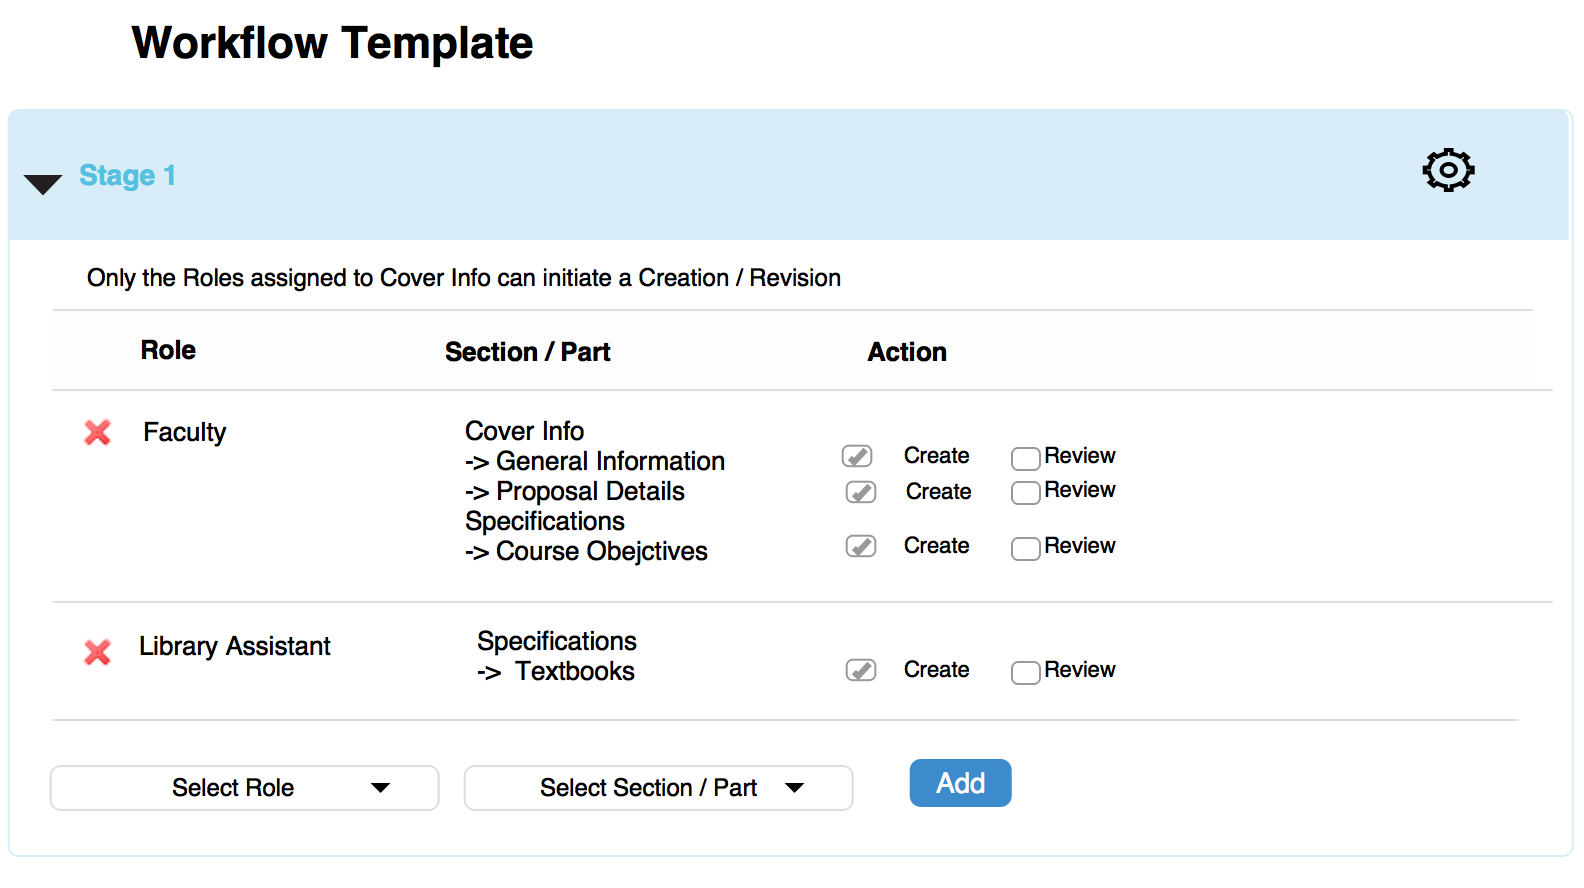
\includegraphics[width=125mm,scale=1]{Capitulos/DesarrollodelaAplicacion/Imagenes/workflow_stage}
\caption{Mockup de la pantalla de plantillas soportando las etapas.}
  \label{workflow_stage}
\end{figure}

\begin{figure}[H]
\centering
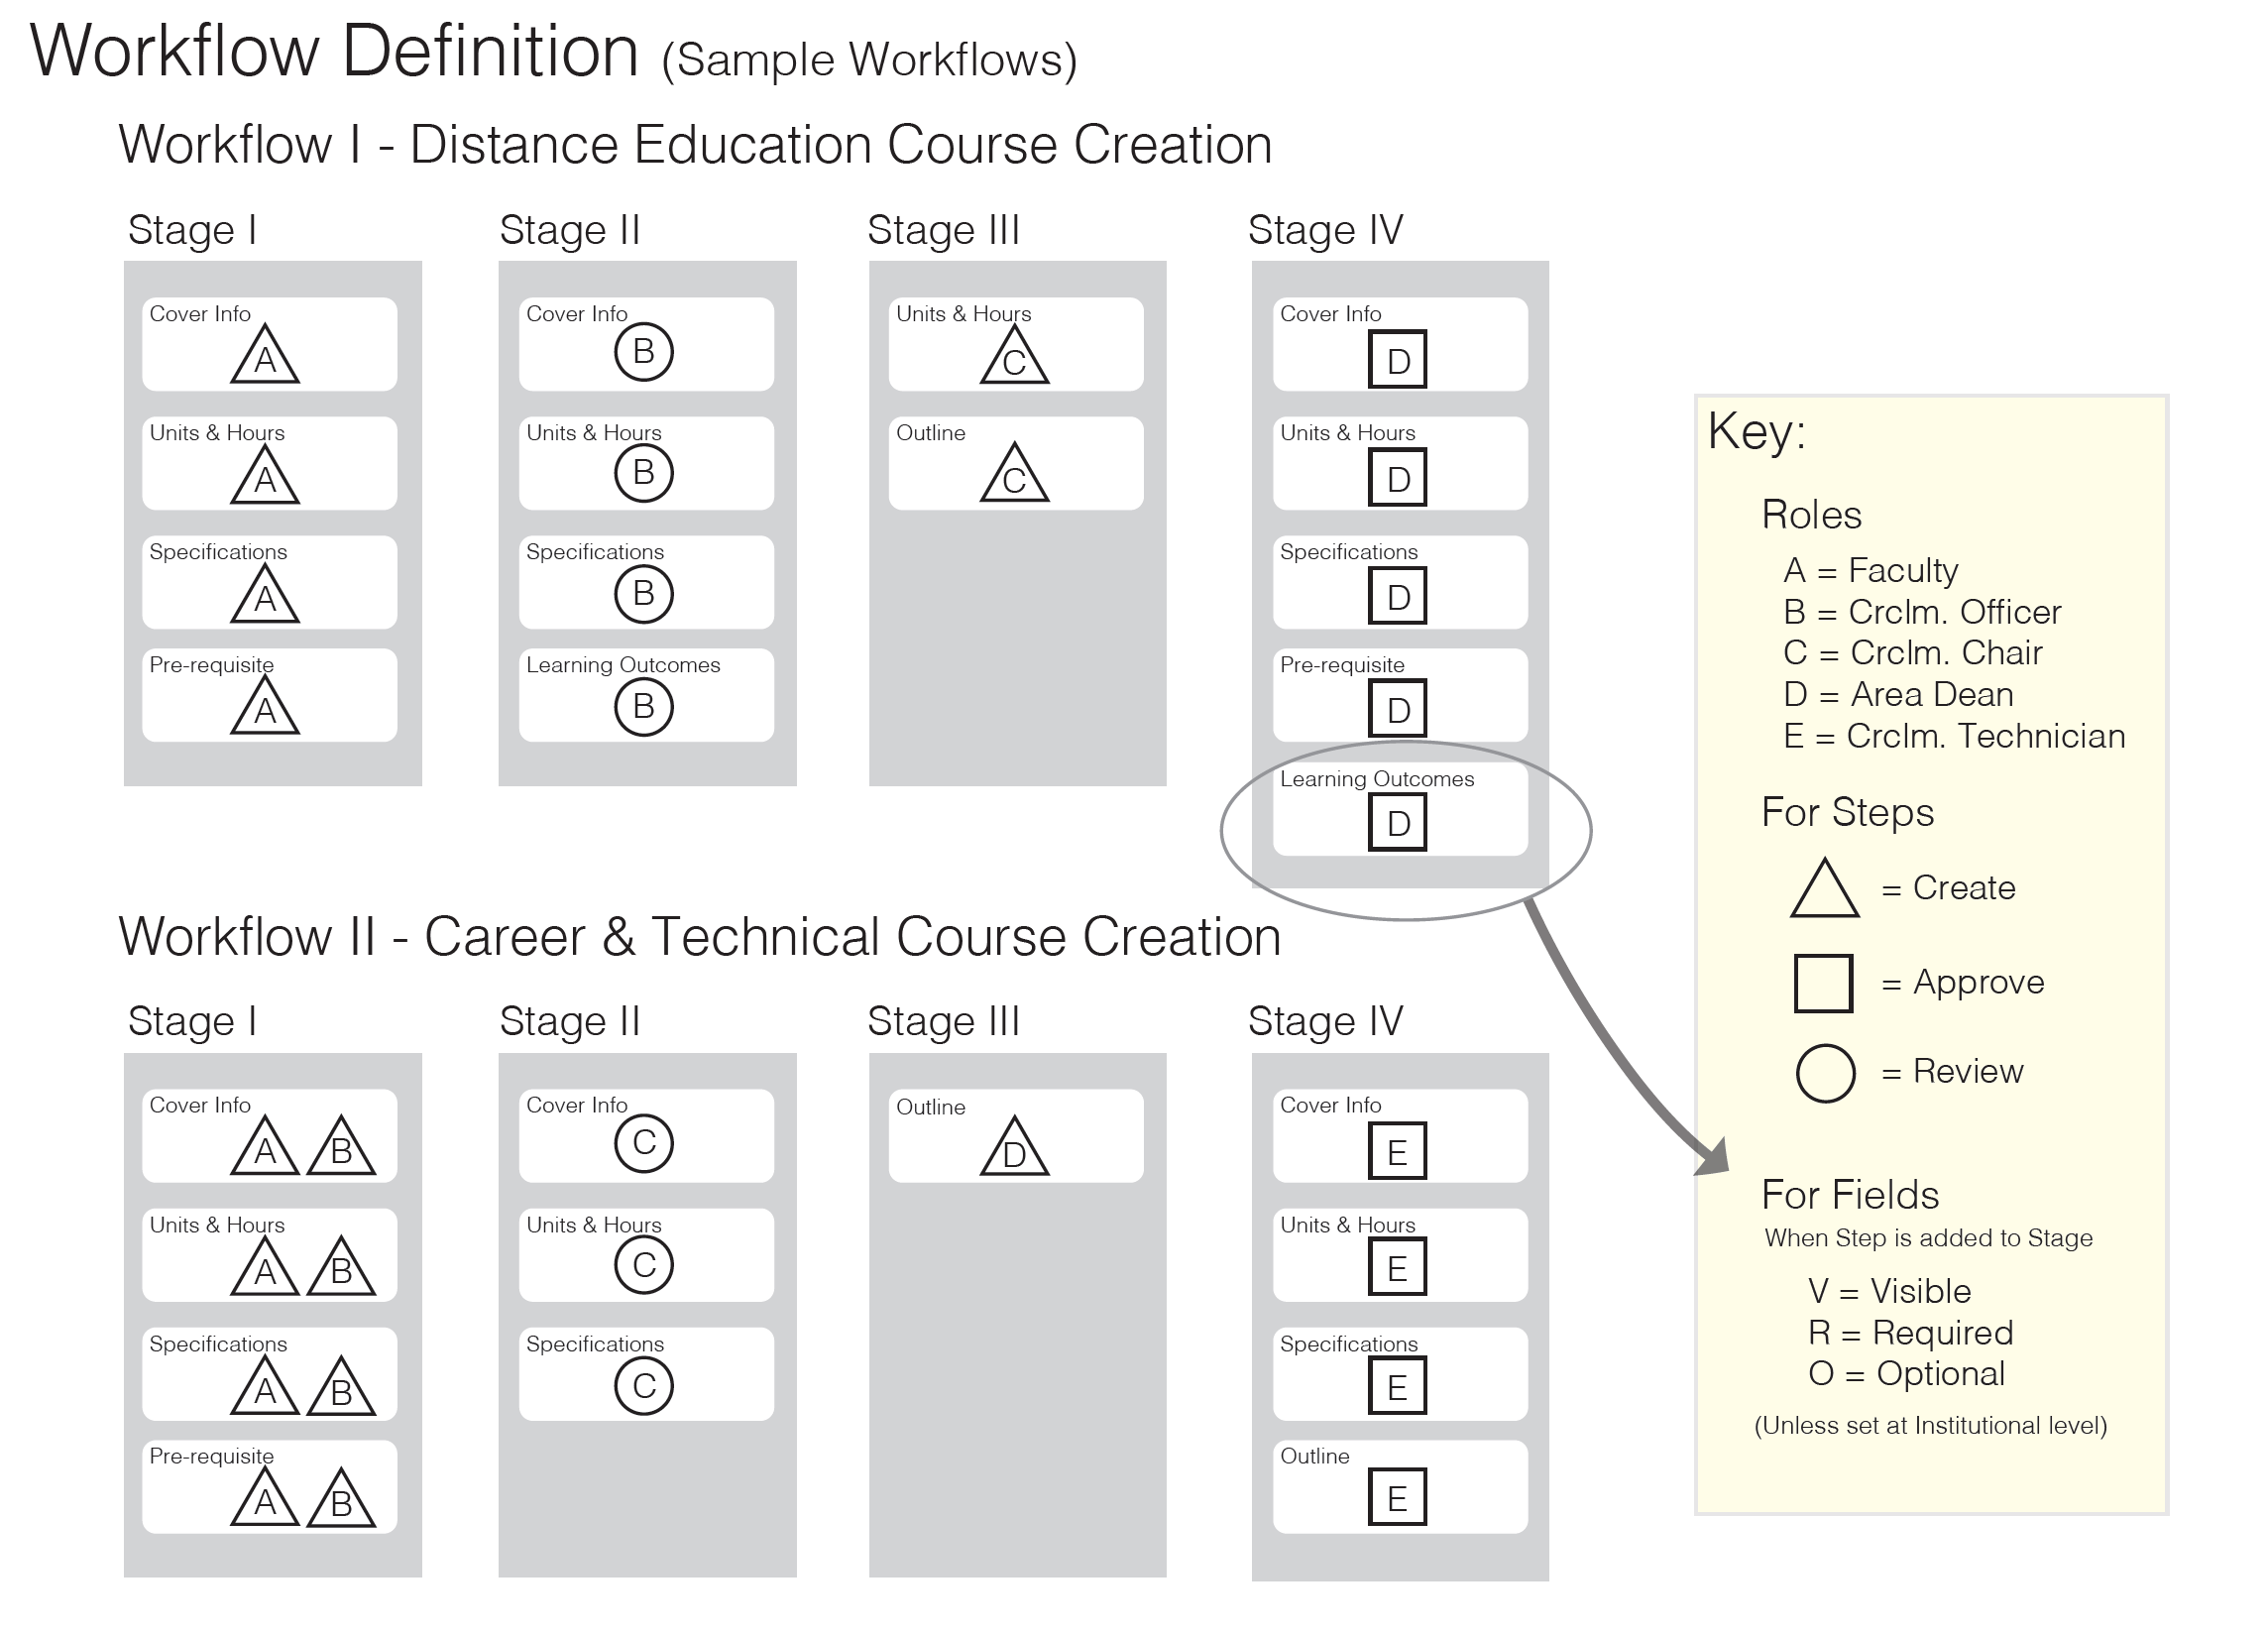
\includegraphics[width=125mm,scale=1]{Capitulos/DesarrollodelaAplicacion/Imagenes/workflow_template_stage}
\caption{Mockup de la pantalla de plantillas con etapas por flujo.}
  \label{workflow_template_stage}
\end{figure}

\subsection{Mejora en comportamientos para las etapas por roles}
La historia de usuario tiene como descripción lo siguiente \enquote{\textit{Como coordinador de educación a distancia, yo solo necesito revisar el esquema del curso para aquellos cursos diseñados para educación a distancia}}.

El criterio de aceptación de la historia consistía en permitir que una etapa que no tiene roles asignados sea opcional.

Algunas de las tareas identificadas en la planificación de las iteraciones eran los siguientes:
\begin{itemize}
	\item Diseñar un plan de pruebas, en estas se identifican las posibles zonas afectadas por la nueva funcionalidad.
	\item Actualizar la pantalla de creación de flujos de trabajo.
	\item Actualizar el mecanismo de transición de etapas.
	\item Mejorar la UI de la vista de etapas de flujos.
\end{itemize}

La historia fue finalizada en tres iteraciones con una cantidad de 108 horas cargadas en el sistema.

\subsection{Composición de etapas y partes}
La historia de usuario tiene como descripción lo siguiente \enquote{\textit{Como presidente curricular, me gustaría ser capaz de componer flujos de trabajo de cursos o programas y etapas (incluyendo actores en cada etapa y sus acciones), para que de esa manera se pueda modelar el proceso curricular en la aplicación}}.

Como criterios de aceptación se encuentran los siguientes:
\begin{itemize}
	\item Cada etapa puede contener una o más partes.
	\item Los actores de cada etapa pueden asignarse actiones a cada parte, o a todas.
	\item Etapas equivalentes no pueden bloquearse entre sí. Por ejemplo, si Suzy y Joe son evaluadores de tres partes, Joe no tiene que esperar que Suzy revise la parte 1 antes de que el pueda evaluar la parte 2, es decir, ambos pueden evaluar sus partes en simultáneo.
\end{itemize}

Algunas de las tareas identificadas en la planificación de las iteraciones eran los siguientes:
\begin{itemize}
	\item Diseño de mockups para su aprobación previa al desarrollo.
	\item Diseño e implementación del modelo de datos que soporte la nueva funcionalidad.
	\item Actualizar las plantillas de flujos de trabajo.
	\item Actualizar los flujos de trabajo de cursos y programas.
	\item Actualizar el sistema de notificaciones.
\end{itemize}

La historia fue finalizada en tres iteraciones con una cantidad de 391 horas cargadas en el sistema.

\subsection{Etapas y partes opcionales en la revisión del flujo}
La historia de usuario tiene como descripción lo siguiente \enquote{\textit{Como administrador curricular quiero ser capaz de configurar mi plantilla de flujo de trabajo para que pueda dividir en etapas donde se especifiquen que roles pueden completar que funciona en una o múltiples secciones o partes de mi programa o curso}}.

Como criterios de aceptación se encuentran los siguientes:
\begin{itemize}
	\item Los roles pueden ser configurados para la acción de creación o revisar, o ambos.
	\item El rol de creación lleva el nombre de creador y para la revisión lleva el nombre de evaluador.
\end{itemize}

Algunas de las tareas identificadas en la planificación de las iteraciones eran los siguientes:
\begin{itemize}
	\item Diseñar un plan de pruebas, en estas se identifican las posibles zonas afectadas por la nueva funcionalidad.
	\item Actualizar la pantalla de creación de flujos de trabajo.
	\item Actualizar el mecanismo de transición de etapas.
\end{itemize}

La historia fue finalizada en tres iteraciones con una cantidad de 76 horas cargadas en el sistema.